
% Default to the notebook output style

    


% Inherit from the specified cell style.




    
\documentclass[11pt]{article}

    
    
    \usepackage[T1]{fontenc}
    % Nicer default font than Computer Modern for most use cases
    \usepackage{palatino}

    % Basic figure setup, for now with no caption control since it's done
    % automatically by Pandoc (which extracts ![](path) syntax from Markdown).
    \usepackage{graphicx}
    % We will generate all images so they have a width \maxwidth. This means
    % that they will get their normal width if they fit onto the page, but
    % are scaled down if they would overflow the margins.
    \makeatletter
    \def\maxwidth{\ifdim\Gin@nat@width>\linewidth\linewidth
    \else\Gin@nat@width\fi}
    \makeatother
    \let\Oldincludegraphics\includegraphics
    % Set max figure width to be 80% of text width, for now hardcoded.
    \renewcommand{\includegraphics}[1]{\Oldincludegraphics[width=.8\maxwidth]{#1}}
    % Ensure that by default, figures have no caption (until we provide a
    % proper Figure object with a Caption API and a way to capture that
    % in the conversion process - todo).
    \usepackage{caption}
    \DeclareCaptionLabelFormat{nolabel}{}
    \captionsetup{labelformat=nolabel}

    \usepackage{adjustbox} % Used to constrain images to a maximum size 
    \usepackage{xcolor} % Allow colors to be defined
    \usepackage{enumerate} % Needed for markdown enumerations to work
    \usepackage{geometry} % Used to adjust the document margins
    \usepackage{amsmath} % Equations
    \usepackage{amssymb} % Equations
    \usepackage{textcomp} % defines textquotesingle
    % Hack from http://tex.stackexchange.com/a/47451/13684:
    \AtBeginDocument{%
        \def\PYZsq{\textquotesingle}% Upright quotes in Pygmentized code
    }
    \usepackage{upquote} % Upright quotes for verbatim code
    \usepackage{eurosym} % defines \euro
    \usepackage[mathletters]{ucs} % Extended unicode (utf-8) support
    \usepackage[utf8x]{inputenc} % Allow utf-8 characters in the tex document
    \usepackage{fancyvrb} % verbatim replacement that allows latex
    \usepackage{grffile} % extends the file name processing of package graphics 
                         % to support a larger range 
    % The hyperref package gives us a pdf with properly built
    % internal navigation ('pdf bookmarks' for the table of contents,
    % internal cross-reference links, web links for URLs, etc.)
    \usepackage{hyperref}
    \usepackage{longtable} % longtable support required by pandoc >1.10
    \usepackage{booktabs}  % table support for pandoc > 1.12.2
    \usepackage[normalem]{ulem} % ulem is needed to support strikethroughs (\sout)
                                % normalem makes italics be italics, not underlines
    

    
    
    % Colors for the hyperref package
    \definecolor{urlcolor}{rgb}{0,.145,.698}
    \definecolor{linkcolor}{rgb}{.71,0.21,0.01}
    \definecolor{citecolor}{rgb}{.12,.54,.11}

    % ANSI colors
    \definecolor{ansi-black}{HTML}{3E424D}
    \definecolor{ansi-black-intense}{HTML}{282C36}
    \definecolor{ansi-red}{HTML}{E75C58}
    \definecolor{ansi-red-intense}{HTML}{B22B31}
    \definecolor{ansi-green}{HTML}{00A250}
    \definecolor{ansi-green-intense}{HTML}{007427}
    \definecolor{ansi-yellow}{HTML}{DDB62B}
    \definecolor{ansi-yellow-intense}{HTML}{B27D12}
    \definecolor{ansi-blue}{HTML}{208FFB}
    \definecolor{ansi-blue-intense}{HTML}{0065CA}
    \definecolor{ansi-magenta}{HTML}{D160C4}
    \definecolor{ansi-magenta-intense}{HTML}{A03196}
    \definecolor{ansi-cyan}{HTML}{60C6C8}
    \definecolor{ansi-cyan-intense}{HTML}{258F8F}
    \definecolor{ansi-white}{HTML}{C5C1B4}
    \definecolor{ansi-white-intense}{HTML}{A1A6B2}

    % commands and environments needed by pandoc snippets
    % extracted from the output of `pandoc -s`
    \providecommand{\tightlist}{%
      \setlength{\itemsep}{0pt}\setlength{\parskip}{0pt}}
    \DefineVerbatimEnvironment{Highlighting}{Verbatim}{commandchars=\\\{\}}
    % Add ',fontsize=\small' for more characters per line
    \newenvironment{Shaded}{}{}
    \newcommand{\KeywordTok}[1]{\textcolor[rgb]{0.00,0.44,0.13}{\textbf{{#1}}}}
    \newcommand{\DataTypeTok}[1]{\textcolor[rgb]{0.56,0.13,0.00}{{#1}}}
    \newcommand{\DecValTok}[1]{\textcolor[rgb]{0.25,0.63,0.44}{{#1}}}
    \newcommand{\BaseNTok}[1]{\textcolor[rgb]{0.25,0.63,0.44}{{#1}}}
    \newcommand{\FloatTok}[1]{\textcolor[rgb]{0.25,0.63,0.44}{{#1}}}
    \newcommand{\CharTok}[1]{\textcolor[rgb]{0.25,0.44,0.63}{{#1}}}
    \newcommand{\StringTok}[1]{\textcolor[rgb]{0.25,0.44,0.63}{{#1}}}
    \newcommand{\CommentTok}[1]{\textcolor[rgb]{0.38,0.63,0.69}{\textit{{#1}}}}
    \newcommand{\OtherTok}[1]{\textcolor[rgb]{0.00,0.44,0.13}{{#1}}}
    \newcommand{\AlertTok}[1]{\textcolor[rgb]{1.00,0.00,0.00}{\textbf{{#1}}}}
    \newcommand{\FunctionTok}[1]{\textcolor[rgb]{0.02,0.16,0.49}{{#1}}}
    \newcommand{\RegionMarkerTok}[1]{{#1}}
    \newcommand{\ErrorTok}[1]{\textcolor[rgb]{1.00,0.00,0.00}{\textbf{{#1}}}}
    \newcommand{\NormalTok}[1]{{#1}}
    
    % Additional commands for more recent versions of Pandoc
    \newcommand{\ConstantTok}[1]{\textcolor[rgb]{0.53,0.00,0.00}{{#1}}}
    \newcommand{\SpecialCharTok}[1]{\textcolor[rgb]{0.25,0.44,0.63}{{#1}}}
    \newcommand{\VerbatimStringTok}[1]{\textcolor[rgb]{0.25,0.44,0.63}{{#1}}}
    \newcommand{\SpecialStringTok}[1]{\textcolor[rgb]{0.73,0.40,0.53}{{#1}}}
    \newcommand{\ImportTok}[1]{{#1}}
    \newcommand{\DocumentationTok}[1]{\textcolor[rgb]{0.73,0.13,0.13}{\textit{{#1}}}}
    \newcommand{\AnnotationTok}[1]{\textcolor[rgb]{0.38,0.63,0.69}{\textbf{\textit{{#1}}}}}
    \newcommand{\CommentVarTok}[1]{\textcolor[rgb]{0.38,0.63,0.69}{\textbf{\textit{{#1}}}}}
    \newcommand{\VariableTok}[1]{\textcolor[rgb]{0.10,0.09,0.49}{{#1}}}
    \newcommand{\ControlFlowTok}[1]{\textcolor[rgb]{0.00,0.44,0.13}{\textbf{{#1}}}}
    \newcommand{\OperatorTok}[1]{\textcolor[rgb]{0.40,0.40,0.40}{{#1}}}
    \newcommand{\BuiltInTok}[1]{{#1}}
    \newcommand{\ExtensionTok}[1]{{#1}}
    \newcommand{\PreprocessorTok}[1]{\textcolor[rgb]{0.74,0.48,0.00}{{#1}}}
    \newcommand{\AttributeTok}[1]{\textcolor[rgb]{0.49,0.56,0.16}{{#1}}}
    \newcommand{\InformationTok}[1]{\textcolor[rgb]{0.38,0.63,0.69}{\textbf{\textit{{#1}}}}}
    \newcommand{\WarningTok}[1]{\textcolor[rgb]{0.38,0.63,0.69}{\textbf{\textit{{#1}}}}}
    
    
    % Define a nice break command that doesn't care if a line doesn't already
    % exist.
    \def\br{\hspace*{\fill} \\* }
    % Math Jax compatability definitions
    \def\gt{>}
    \def\lt{<}
    % Document parameters
    \title{Introduction to OOP}
    
    
    

    % Pygments definitions
    
\makeatletter
\def\PY@reset{\let\PY@it=\relax \let\PY@bf=\relax%
    \let\PY@ul=\relax \let\PY@tc=\relax%
    \let\PY@bc=\relax \let\PY@ff=\relax}
\def\PY@tok#1{\csname PY@tok@#1\endcsname}
\def\PY@toks#1+{\ifx\relax#1\empty\else%
    \PY@tok{#1}\expandafter\PY@toks\fi}
\def\PY@do#1{\PY@bc{\PY@tc{\PY@ul{%
    \PY@it{\PY@bf{\PY@ff{#1}}}}}}}
\def\PY#1#2{\PY@reset\PY@toks#1+\relax+\PY@do{#2}}

\expandafter\def\csname PY@tok@kr\endcsname{\let\PY@bf=\textbf\def\PY@tc##1{\textcolor[rgb]{0.00,0.50,0.00}{##1}}}
\expandafter\def\csname PY@tok@si\endcsname{\let\PY@bf=\textbf\def\PY@tc##1{\textcolor[rgb]{0.73,0.40,0.53}{##1}}}
\expandafter\def\csname PY@tok@gu\endcsname{\let\PY@bf=\textbf\def\PY@tc##1{\textcolor[rgb]{0.50,0.00,0.50}{##1}}}
\expandafter\def\csname PY@tok@kt\endcsname{\def\PY@tc##1{\textcolor[rgb]{0.69,0.00,0.25}{##1}}}
\expandafter\def\csname PY@tok@s1\endcsname{\def\PY@tc##1{\textcolor[rgb]{0.73,0.13,0.13}{##1}}}
\expandafter\def\csname PY@tok@mh\endcsname{\def\PY@tc##1{\textcolor[rgb]{0.40,0.40,0.40}{##1}}}
\expandafter\def\csname PY@tok@nf\endcsname{\def\PY@tc##1{\textcolor[rgb]{0.00,0.00,1.00}{##1}}}
\expandafter\def\csname PY@tok@sb\endcsname{\def\PY@tc##1{\textcolor[rgb]{0.73,0.13,0.13}{##1}}}
\expandafter\def\csname PY@tok@gt\endcsname{\def\PY@tc##1{\textcolor[rgb]{0.00,0.27,0.87}{##1}}}
\expandafter\def\csname PY@tok@gp\endcsname{\let\PY@bf=\textbf\def\PY@tc##1{\textcolor[rgb]{0.00,0.00,0.50}{##1}}}
\expandafter\def\csname PY@tok@bp\endcsname{\def\PY@tc##1{\textcolor[rgb]{0.00,0.50,0.00}{##1}}}
\expandafter\def\csname PY@tok@il\endcsname{\def\PY@tc##1{\textcolor[rgb]{0.40,0.40,0.40}{##1}}}
\expandafter\def\csname PY@tok@nd\endcsname{\def\PY@tc##1{\textcolor[rgb]{0.67,0.13,1.00}{##1}}}
\expandafter\def\csname PY@tok@w\endcsname{\def\PY@tc##1{\textcolor[rgb]{0.73,0.73,0.73}{##1}}}
\expandafter\def\csname PY@tok@nt\endcsname{\let\PY@bf=\textbf\def\PY@tc##1{\textcolor[rgb]{0.00,0.50,0.00}{##1}}}
\expandafter\def\csname PY@tok@cp\endcsname{\def\PY@tc##1{\textcolor[rgb]{0.74,0.48,0.00}{##1}}}
\expandafter\def\csname PY@tok@mf\endcsname{\def\PY@tc##1{\textcolor[rgb]{0.40,0.40,0.40}{##1}}}
\expandafter\def\csname PY@tok@nn\endcsname{\let\PY@bf=\textbf\def\PY@tc##1{\textcolor[rgb]{0.00,0.00,1.00}{##1}}}
\expandafter\def\csname PY@tok@ss\endcsname{\def\PY@tc##1{\textcolor[rgb]{0.10,0.09,0.49}{##1}}}
\expandafter\def\csname PY@tok@ni\endcsname{\let\PY@bf=\textbf\def\PY@tc##1{\textcolor[rgb]{0.60,0.60,0.60}{##1}}}
\expandafter\def\csname PY@tok@na\endcsname{\def\PY@tc##1{\textcolor[rgb]{0.49,0.56,0.16}{##1}}}
\expandafter\def\csname PY@tok@sx\endcsname{\def\PY@tc##1{\textcolor[rgb]{0.00,0.50,0.00}{##1}}}
\expandafter\def\csname PY@tok@mb\endcsname{\def\PY@tc##1{\textcolor[rgb]{0.40,0.40,0.40}{##1}}}
\expandafter\def\csname PY@tok@s\endcsname{\def\PY@tc##1{\textcolor[rgb]{0.73,0.13,0.13}{##1}}}
\expandafter\def\csname PY@tok@gd\endcsname{\def\PY@tc##1{\textcolor[rgb]{0.63,0.00,0.00}{##1}}}
\expandafter\def\csname PY@tok@go\endcsname{\def\PY@tc##1{\textcolor[rgb]{0.53,0.53,0.53}{##1}}}
\expandafter\def\csname PY@tok@err\endcsname{\def\PY@bc##1{\setlength{\fboxsep}{0pt}\fcolorbox[rgb]{1.00,0.00,0.00}{1,1,1}{\strut ##1}}}
\expandafter\def\csname PY@tok@no\endcsname{\def\PY@tc##1{\textcolor[rgb]{0.53,0.00,0.00}{##1}}}
\expandafter\def\csname PY@tok@se\endcsname{\let\PY@bf=\textbf\def\PY@tc##1{\textcolor[rgb]{0.73,0.40,0.13}{##1}}}
\expandafter\def\csname PY@tok@mi\endcsname{\def\PY@tc##1{\textcolor[rgb]{0.40,0.40,0.40}{##1}}}
\expandafter\def\csname PY@tok@cs\endcsname{\let\PY@it=\textit\def\PY@tc##1{\textcolor[rgb]{0.25,0.50,0.50}{##1}}}
\expandafter\def\csname PY@tok@sh\endcsname{\def\PY@tc##1{\textcolor[rgb]{0.73,0.13,0.13}{##1}}}
\expandafter\def\csname PY@tok@gi\endcsname{\def\PY@tc##1{\textcolor[rgb]{0.00,0.63,0.00}{##1}}}
\expandafter\def\csname PY@tok@vc\endcsname{\def\PY@tc##1{\textcolor[rgb]{0.10,0.09,0.49}{##1}}}
\expandafter\def\csname PY@tok@c1\endcsname{\let\PY@it=\textit\def\PY@tc##1{\textcolor[rgb]{0.25,0.50,0.50}{##1}}}
\expandafter\def\csname PY@tok@nv\endcsname{\def\PY@tc##1{\textcolor[rgb]{0.10,0.09,0.49}{##1}}}
\expandafter\def\csname PY@tok@nl\endcsname{\def\PY@tc##1{\textcolor[rgb]{0.63,0.63,0.00}{##1}}}
\expandafter\def\csname PY@tok@gs\endcsname{\let\PY@bf=\textbf}
\expandafter\def\csname PY@tok@k\endcsname{\let\PY@bf=\textbf\def\PY@tc##1{\textcolor[rgb]{0.00,0.50,0.00}{##1}}}
\expandafter\def\csname PY@tok@vi\endcsname{\def\PY@tc##1{\textcolor[rgb]{0.10,0.09,0.49}{##1}}}
\expandafter\def\csname PY@tok@mo\endcsname{\def\PY@tc##1{\textcolor[rgb]{0.40,0.40,0.40}{##1}}}
\expandafter\def\csname PY@tok@kn\endcsname{\let\PY@bf=\textbf\def\PY@tc##1{\textcolor[rgb]{0.00,0.50,0.00}{##1}}}
\expandafter\def\csname PY@tok@ch\endcsname{\let\PY@it=\textit\def\PY@tc##1{\textcolor[rgb]{0.25,0.50,0.50}{##1}}}
\expandafter\def\csname PY@tok@nc\endcsname{\let\PY@bf=\textbf\def\PY@tc##1{\textcolor[rgb]{0.00,0.00,1.00}{##1}}}
\expandafter\def\csname PY@tok@nb\endcsname{\def\PY@tc##1{\textcolor[rgb]{0.00,0.50,0.00}{##1}}}
\expandafter\def\csname PY@tok@kc\endcsname{\let\PY@bf=\textbf\def\PY@tc##1{\textcolor[rgb]{0.00,0.50,0.00}{##1}}}
\expandafter\def\csname PY@tok@m\endcsname{\def\PY@tc##1{\textcolor[rgb]{0.40,0.40,0.40}{##1}}}
\expandafter\def\csname PY@tok@sd\endcsname{\let\PY@it=\textit\def\PY@tc##1{\textcolor[rgb]{0.73,0.13,0.13}{##1}}}
\expandafter\def\csname PY@tok@vg\endcsname{\def\PY@tc##1{\textcolor[rgb]{0.10,0.09,0.49}{##1}}}
\expandafter\def\csname PY@tok@o\endcsname{\def\PY@tc##1{\textcolor[rgb]{0.40,0.40,0.40}{##1}}}
\expandafter\def\csname PY@tok@ne\endcsname{\let\PY@bf=\textbf\def\PY@tc##1{\textcolor[rgb]{0.82,0.25,0.23}{##1}}}
\expandafter\def\csname PY@tok@sr\endcsname{\def\PY@tc##1{\textcolor[rgb]{0.73,0.40,0.53}{##1}}}
\expandafter\def\csname PY@tok@kd\endcsname{\let\PY@bf=\textbf\def\PY@tc##1{\textcolor[rgb]{0.00,0.50,0.00}{##1}}}
\expandafter\def\csname PY@tok@c\endcsname{\let\PY@it=\textit\def\PY@tc##1{\textcolor[rgb]{0.25,0.50,0.50}{##1}}}
\expandafter\def\csname PY@tok@gh\endcsname{\let\PY@bf=\textbf\def\PY@tc##1{\textcolor[rgb]{0.00,0.00,0.50}{##1}}}
\expandafter\def\csname PY@tok@gr\endcsname{\def\PY@tc##1{\textcolor[rgb]{1.00,0.00,0.00}{##1}}}
\expandafter\def\csname PY@tok@cm\endcsname{\let\PY@it=\textit\def\PY@tc##1{\textcolor[rgb]{0.25,0.50,0.50}{##1}}}
\expandafter\def\csname PY@tok@cpf\endcsname{\let\PY@it=\textit\def\PY@tc##1{\textcolor[rgb]{0.25,0.50,0.50}{##1}}}
\expandafter\def\csname PY@tok@ge\endcsname{\let\PY@it=\textit}
\expandafter\def\csname PY@tok@ow\endcsname{\let\PY@bf=\textbf\def\PY@tc##1{\textcolor[rgb]{0.67,0.13,1.00}{##1}}}
\expandafter\def\csname PY@tok@sc\endcsname{\def\PY@tc##1{\textcolor[rgb]{0.73,0.13,0.13}{##1}}}
\expandafter\def\csname PY@tok@kp\endcsname{\def\PY@tc##1{\textcolor[rgb]{0.00,0.50,0.00}{##1}}}
\expandafter\def\csname PY@tok@s2\endcsname{\def\PY@tc##1{\textcolor[rgb]{0.73,0.13,0.13}{##1}}}

\def\PYZbs{\char`\\}
\def\PYZus{\char`\_}
\def\PYZob{\char`\{}
\def\PYZcb{\char`\}}
\def\PYZca{\char`\^}
\def\PYZam{\char`\&}
\def\PYZlt{\char`\<}
\def\PYZgt{\char`\>}
\def\PYZsh{\char`\#}
\def\PYZpc{\char`\%}
\def\PYZdl{\char`\$}
\def\PYZhy{\char`\-}
\def\PYZsq{\char`\'}
\def\PYZdq{\char`\"}
\def\PYZti{\char`\~}
% for compatibility with earlier versions
\def\PYZat{@}
\def\PYZlb{[}
\def\PYZrb{]}
\makeatother


    % Exact colors from NB
    \definecolor{incolor}{rgb}{0.0, 0.0, 0.5}
    \definecolor{outcolor}{rgb}{0.545, 0.0, 0.0}



    
    % Prevent overflowing lines due to hard-to-break entities
    \sloppy 
    % Setup hyperref package
    \hypersetup{
      breaklinks=true,  % so long urls are correctly broken across lines
      colorlinks=true,
      urlcolor=urlcolor,
      linkcolor=linkcolor,
      citecolor=citecolor,
      }
    % Slightly bigger margins than the latex defaults
    
    \geometry{verbose,tmargin=1in,bmargin=1in,lmargin=1in,rmargin=1in}
    
    

    \begin{document}
    
    
    \maketitle
    
    

    
    \subsection{Introduction to Object Oriented Programming with
Python}\label{introduction-to-object-oriented-programming-with-python}

This prepares you for a 2 day challenge. The goals:

\begin{enumerate}
\def\labelenumi{\arabic{enumi}.}
\tightlist
\item
  Be able to write Python code;
\item
  Understand the ideas behind object oriented programming.
\end{enumerate}

\subsubsection{Basic Python}\label{basic-python}

\begin{enumerate}
\def\labelenumi{\arabic{enumi}.}
\tightlist
\item
  Variables;
\item
  Flow Control;
\item
  Functions;
\item
  Data structure.
\end{enumerate}

\subsubsection{Basic Object Oriented
Programming}\label{basic-object-oriented-programming}

\begin{enumerate}
\def\labelenumi{\arabic{enumi}.}
\tightlist
\item
  Classes;
\item
  Attributes;
\item
  Methods;
\item
  Inheritance.
\end{enumerate}

\subsubsection{The Challenge}\label{the-challenge}

\begin{enumerate}
\def\labelenumi{\arabic{enumi}.}
\tightlist
\item
  End of the day Thursday: Initial Feedback;
\item
  End of the day Friday: results.
\end{enumerate}

\subsection{Overview of Python}\label{overview-of-python}

What is Python?

Python is a programming language. There are various other programming
languages:

Java C C++ Ruby VBA and many more. A programming language allows you to
write a program which is a sequence of instructions that specifies how
to perform a computation.

When writing a program you need two things:

Something to save the code (a text editor for example) Something to run
the code We will be using a combination of these 2 things called
notebooks.

\subsection{Installing Python}\label{installing-python}

There are various distributions of Python, we will use Anaconda which
comes packaged with a variety of other useful tools (including the
notebooks I mentioned above).

To install it on your personal machine follow these steps:

Go to this webpage: https://www.continuum.io/downloads.

Identify and download the version of \textbf{Python 3} for your
operating system (Windows, Mac OSX, Linux). Run the installer. We will
use a Jupyter notebook which runs in your browser. To open a local
server find the Continuum navigator and click on Jupyter. You do not
need to be connected to the internet to use this.

\subsection{Interacting with Python}\label{interacting-with-python}

Once you have installed Anaconda, you will now have Python on your
machine. You can interact with Python in multiple ways:

\subsubsection{The Python shell}\label{the-python-shell}

\begin{itemize}
\item
  On Windows open a ``Command Prompt'':
\item
  On Mac OS or Linux open a ``Terminal'':
\end{itemize}

This is a simple utility that allows you to give commands to your
computer. In there type:

\begin{Shaded}
\begin{Highlighting}[]
\KeywordTok{python}
\end{Highlighting}
\end{Shaded}

This should then look something like:

\begin{Shaded}
\begin{Highlighting}[]
\NormalTok{Python }\FloatTok{3.5.2} \OperatorTok{|}\NormalTok{Anaconda }\FloatTok{4.2.0} \NormalTok{(}\DecValTok{64}\OperatorTok{-}\NormalTok{bit)}\OperatorTok{|} \NormalTok{(default, Jul  }\DecValTok{2} \DecValTok{2016}\NormalTok{, }\DecValTok{17}\NormalTok{:}\DecValTok{53}\NormalTok{:}\DecValTok{06}\NormalTok{) }
\NormalTok{[GCC }\FloatTok{4.4.7} \DecValTok{20120313} \NormalTok{(Red Hat }\FloatTok{4.4.7}\DecValTok{-1}\NormalTok{)] on linux}
\NormalTok{Type }\StringTok{"help"}\NormalTok{, }\StringTok{"copyright"}\NormalTok{, }\StringTok{"credits"} \OperatorTok{or} \StringTok{"license"} \ControlFlowTok{for} \NormalTok{more information.}
\OperatorTok{>>>} 
\end{Highlighting}
\end{Shaded}

The \texttt{\textgreater{}\textgreater{}\textgreater{}} is a prompt for
you to type a command. Let us carry out a straightforward addition:

\begin{Shaded}
\begin{Highlighting}[]
\OperatorTok{>>>} \DecValTok{2} \OperatorTok{+} \DecValTok{2}
\end{Highlighting}
\end{Shaded}

and press \texttt{ENTER}:

\begin{Shaded}
\begin{Highlighting}[]
\OperatorTok{>>>} \DecValTok{2} \OperatorTok{+} \DecValTok{2}
\DecValTok{4}
\end{Highlighting}
\end{Shaded}

\textbf{This is not a very efficient and practical way of using Python.}
We will instead learn to use a \href{http://jupyter.org/}{Jupyter
notebook}.

\subsubsection{Jupyter notebooks}\label{jupyter-notebooks}

If you are still in the Python shell (with a
\texttt{\textgreater{}\textgreater{}\textgreater{}} waiting for you to
give a command) then type:

\begin{Shaded}
\begin{Highlighting}[]
\OperatorTok{>>>} \NormalTok{exit()}
\end{Highlighting}
\end{Shaded}

This will leave the prompt and you will now be back at the Command
Prompt or the Terminal window. Here simply type:

\begin{Shaded}
\begin{Highlighting}[]
\KeywordTok{jupyter} \NormalTok{notebook}
\end{Highlighting}
\end{Shaded}

After a little moment this will open a Jupyter notebook page in a
browser. Note that this is all just running on your computer and you do
not need to be connected to the internet to use a Jupyter notebook.

Click on \texttt{New} and create a notebook: we can start to write code
now.

\subsubsection{Basic Python}\label{basic-python-1}

Write \texttt{2\ +\ 2} in a cell and press \texttt{shift\ +\ Enter}:

    \begin{Verbatim}[commandchars=\\\{\}]
{\color{incolor}In [{\color{incolor}2}]:} \PY{l+m+mi}{2} \PY{o}{+} \PY{l+m+mi}{2}
\end{Verbatim}

            \begin{Verbatim}[commandchars=\\\{\}]
{\color{outcolor}Out[{\color{outcolor}2}]:} 4
\end{Verbatim}
        
    \subsection{Variables}\label{variables}

\subsubsection{Character variables:}\label{character-variables}

    \begin{Verbatim}[commandchars=\\\{\}]
{\color{incolor}In [{\color{incolor}3}]:} \PY{n}{string} \PY{o}{=} \PY{l+s+s2}{\PYZdq{}}\PY{l+s+s2}{Hello world}\PY{l+s+s2}{\PYZdq{}}
        \PY{n}{string}
\end{Verbatim}

            \begin{Verbatim}[commandchars=\\\{\}]
{\color{outcolor}Out[{\color{outcolor}3}]:} 'Hello world'
\end{Verbatim}
        
    \subsubsection{Numeric variables:}\label{numeric-variables}

    \begin{Verbatim}[commandchars=\\\{\}]
{\color{incolor}In [{\color{incolor}4}]:} \PY{n}{num\PYZus{}1} \PY{o}{=} \PY{l+m+mi}{2}
        \PY{n}{num\PYZus{}2} \PY{o}{=} \PY{l+m+mf}{3.5}
        \PY{n}{num\PYZus{}1} \PY{o}{+} \PY{n}{num\PYZus{}2}
\end{Verbatim}

            \begin{Verbatim}[commandchars=\\\{\}]
{\color{outcolor}Out[{\color{outcolor}4}]:} 5.5
\end{Verbatim}
        
    \subsubsection{String manipulation}\label{string-manipulation}

    \begin{Verbatim}[commandchars=\\\{\}]
{\color{incolor}In [{\color{incolor}7}]:} \PY{c+c1}{\PYZsh{}We define a variable called String }
        \PY{c+c1}{\PYZsh{} (note that \PYZsh{} allows me to comment my code)}
        \PY{n}{string} \PY{o}{=} \PY{l+s+s2}{\PYZdq{}}\PY{l+s+s2}{My name is Vince}\PY{l+s+s2}{\PYZdq{}}
        \PY{c+c1}{\PYZsh{}Let\PYZsq{}s get the 5th letter of String }
        \PY{c+c1}{\PYZsh{} (Note that Python starts counting at 0):}
        \PY{n}{string}\PY{p}{[}\PY{l+m+mi}{4}\PY{p}{]}
\end{Verbatim}

            \begin{Verbatim}[commandchars=\\\{\}]
{\color{outcolor}Out[{\color{outcolor}7}]:} 'a'
\end{Verbatim}
        
    \begin{Verbatim}[commandchars=\\\{\}]
{\color{incolor}In [{\color{incolor}8}]:} \PY{n}{string}\PY{p}{[}\PY{l+m+mi}{1}\PY{p}{:}\PY{l+m+mi}{4}\PY{p}{]}
\end{Verbatim}

            \begin{Verbatim}[commandchars=\\\{\}]
{\color{outcolor}Out[{\color{outcolor}8}]:} 'y n'
\end{Verbatim}
        
    \begin{Verbatim}[commandchars=\\\{\}]
{\color{incolor}In [{\color{incolor}11}]:} \PY{n}{index\PYZus{}of\PYZus{}v} \PY{o}{=} \PY{n}{string}\PY{o}{.}\PY{n}{index}\PY{p}{(}\PY{l+s+s2}{\PYZdq{}}\PY{l+s+s2}{V}\PY{l+s+s2}{\PYZdq{}}\PY{p}{)}
         \PY{n}{index\PYZus{}of\PYZus{}v}
\end{Verbatim}

            \begin{Verbatim}[commandchars=\\\{\}]
{\color{outcolor}Out[{\color{outcolor}11}]:} 11
\end{Verbatim}
        
    \begin{Verbatim}[commandchars=\\\{\}]
{\color{incolor}In [{\color{incolor}12}]:} \PY{n}{string}\PY{p}{[}\PY{n}{index\PYZus{}of\PYZus{}v}\PY{p}{:}\PY{p}{]}
         \PY{n}{string}\PY{p}{[}\PY{p}{:}\PY{n}{index\PYZus{}of\PYZus{}v}\PY{p}{]}
\end{Verbatim}

            \begin{Verbatim}[commandchars=\\\{\}]
{\color{outcolor}Out[{\color{outcolor}12}]:} 'My name is '
\end{Verbatim}
        
    \subsubsection{Numeric manipulation}\label{numeric-manipulation}

    \begin{Verbatim}[commandchars=\\\{\}]
{\color{incolor}In [{\color{incolor}13}]:} \PY{n}{num} \PY{o}{=} \PY{l+m+mi}{3}
         
         \PY{c+c1}{\PYZsh{} The following two lines are equivalent}
         \PY{n}{num} \PY{o}{=} \PY{n}{num} \PY{o}{+} \PY{l+m+mi}{1}
         \PY{n}{num} \PY{o}{+}\PY{o}{=} \PY{l+m+mi}{1}
         \PY{n}{num}
\end{Verbatim}

            \begin{Verbatim}[commandchars=\\\{\}]
{\color{outcolor}Out[{\color{outcolor}13}]:} 5
\end{Verbatim}
        
    \begin{Verbatim}[commandchars=\\\{\}]
{\color{incolor}In [{\color{incolor}14}]:} \PY{n}{num} \PY{o}{\PYZhy{}}\PY{o}{=} \PY{l+m+mi}{2}
         \PY{n}{num} \PY{o}{*}\PY{o}{=} \PY{l+m+mi}{3}
         \PY{n}{num} \PY{o}{*}\PY{o}{*}\PY{o}{=} \PY{l+m+mi}{2}
         \PY{n}{num}
\end{Verbatim}

            \begin{Verbatim}[commandchars=\\\{\}]
{\color{outcolor}Out[{\color{outcolor}14}]:} 81
\end{Verbatim}
        
    \subsection{Flow control}\label{flow-control}

\begin{itemize}
\tightlist
\item
  In Python indentation is important!
\item
  In all languages indentation is good practice, in Python it is a
  requirement.
\end{itemize}

\subsubsection{If statements}\label{if-statements}

    \begin{Verbatim}[commandchars=\\\{\}]
{\color{incolor}In [{\color{incolor}23}]:} \PY{n}{n} \PY{o}{=} \PY{l+m+mi}{11} 
         \PY{k}{if} \PY{n}{n} \PY{o}{\PYZlt{}}\PY{o}{=} \PY{l+m+mi}{5}\PY{p}{:}
             \PY{n}{value} \PY{o}{=} \PY{l+m+mi}{1}
         \PY{k}{elif} \PY{n}{n} \PY{o}{\PYZpc{}} \PY{l+m+mi}{2} \PY{o}{==} \PY{l+m+mi}{0}\PY{p}{:}  
             \PY{n}{value} \PY{o}{=} \PY{l+m+mi}{2}
         \PY{k}{else}\PY{p}{:} 
             \PY{n}{value} \PY{o}{=} \PY{l+m+mi}{3}
         \PY{n}{value}
\end{Verbatim}

            \begin{Verbatim}[commandchars=\\\{\}]
{\color{outcolor}Out[{\color{outcolor}23}]:} 3
\end{Verbatim}
        
    \subsubsection{While loops}\label{while-loops}

    \begin{Verbatim}[commandchars=\\\{\}]
{\color{incolor}In [{\color{incolor}25}]:} \PY{n}{count} \PY{o}{=} \PY{l+m+mi}{0}  
         \PY{n}{total} \PY{o}{=} \PY{l+m+mi}{0} 
         \PY{k}{while} \PY{n}{count} \PY{o}{\PYZlt{}} \PY{l+m+mi}{10}\PY{p}{:} 
             \PY{n}{count} \PY{o}{+}\PY{o}{=} \PY{l+m+mi}{1}  
             \PY{n}{total} \PY{o}{+}\PY{o}{=} \PY{n}{count} 
         \PY{n}{total}
\end{Verbatim}

            \begin{Verbatim}[commandchars=\\\{\}]
{\color{outcolor}Out[{\color{outcolor}25}]:} 55
\end{Verbatim}
        
    \subsubsection{For loops}\label{for-loops}

    \begin{Verbatim}[commandchars=\\\{\}]
{\color{incolor}In [{\color{incolor}26}]:} \PY{k}{for} \PY{n}{i} \PY{o+ow}{in} \PY{p}{[}\PY{l+m+mi}{1}\PY{p}{,} \PY{l+m+mi}{2}\PY{p}{,} \PY{l+m+mi}{3}\PY{p}{,} \PY{l+m+mi}{4}\PY{p}{]}\PY{p}{:}
             \PY{n+nb}{print}\PY{p}{(}\PY{n}{i}\PY{p}{)}
\end{Verbatim}

    \begin{Verbatim}[commandchars=\\\{\}]
1
2
3
4

    \end{Verbatim}

    \begin{Verbatim}[commandchars=\\\{\}]
{\color{incolor}In [{\color{incolor}30}]:} \PY{k}{for} \PY{n}{subject} \PY{o+ow}{in} \PY{p}{[}\PY{l+s+s2}{\PYZdq{}}\PY{l+s+s2}{Queueing Theory}\PY{l+s+s2}{\PYZdq{}}\PY{p}{,} \PY{l+s+s2}{\PYZdq{}}\PY{l+s+s2}{Game Theory}\PY{l+s+s2}{\PYZdq{}}\PY{p}{,} 
                         \PY{l+s+s2}{\PYZdq{}}\PY{l+s+s2}{Inventory Theory}\PY{l+s+s2}{\PYZdq{}}\PY{p}{,} \PY{l+s+s2}{\PYZdq{}}\PY{l+s+s2}{Reliability Theory}\PY{l+s+s2}{\PYZdq{}}\PY{p}{,} 
                         \PY{l+s+s2}{\PYZdq{}}\PY{l+s+s2}{Project Management}\PY{l+s+s2}{\PYZdq{}}\PY{p}{,} \PY{l+s+s2}{\PYZdq{}}\PY{l+s+s2}{Decision Analysis}\PY{l+s+s2}{\PYZdq{}}\PY{p}{]}\PY{p}{:}
             \PY{k}{if} \PY{l+s+s2}{\PYZdq{}}\PY{l+s+s2}{Theory}\PY{l+s+s2}{\PYZdq{}} \PY{o+ow}{in} \PY{n}{subject}\PY{p}{:}
                 \PY{n+nb}{print}\PY{p}{(}\PY{n}{subject}\PY{p}{)}
\end{Verbatim}

    \begin{Verbatim}[commandchars=\\\{\}]
Queueing Theory
Game Theory
Inventory Theory
Reliability Theory

    \end{Verbatim}

    \subsection{Functions}\label{functions}

    \begin{Verbatim}[commandchars=\\\{\}]
{\color{incolor}In [{\color{incolor}31}]:} \PY{c+c1}{\PYZsh{}To create a function we use the \PYZsq{}def\PYZsq{} statement:}
         \PY{k}{def} \PY{n+nf}{hi}\PY{p}{(}\PY{p}{)}\PY{p}{:}
             \PY{l+s+sd}{\PYZdq{}\PYZdq{}\PYZdq{}}
         \PY{l+s+sd}{    This function simply prints a short statement. }
         \PY{l+s+sd}{    }
         \PY{l+s+sd}{    This is a shorter way of writing documentation, }
         \PY{l+s+sd}{    it is good practice to always include a }
         \PY{l+s+sd}{    description of what a function does.}
         \PY{l+s+sd}{    \PYZdq{}\PYZdq{}\PYZdq{}}
             \PY{n+nb}{print}\PY{p}{(}\PY{l+s+s2}{\PYZdq{}}\PY{l+s+s2}{Hello everybody!}\PY{l+s+s2}{\PYZdq{}}\PY{p}{)}
         
         \PY{n}{hi}\PY{p}{(}\PY{p}{)}
\end{Verbatim}

    \begin{Verbatim}[commandchars=\\\{\}]
Hello everybody!

    \end{Verbatim}

    \begin{Verbatim}[commandchars=\\\{\}]
{\color{incolor}In [{\color{incolor}34}]:} \PY{k}{def} \PY{n+nf}{fibonacci}\PY{p}{(}\PY{n}{n}\PY{p}{)}\PY{p}{:}
             \PY{l+s+sd}{\PYZdq{}\PYZdq{}\PYZdq{}}
         \PY{l+s+sd}{    This returns the nth Fibonacci number.}
         \PY{l+s+sd}{    \PYZdq{}\PYZdq{}\PYZdq{}}
             \PY{k}{if} \PY{n}{n} \PY{o}{==} \PY{l+m+mi}{0}\PY{p}{:}
                 \PY{k}{return} \PY{l+m+mi}{0}
             \PY{k}{if} \PY{n}{n} \PY{o}{==} \PY{l+m+mi}{1}\PY{p}{:}
                 \PY{k}{return} \PY{l+m+mi}{1}
             \PY{k}{return} \PY{n}{fibonacci}\PY{p}{(}\PY{n}{n} \PY{o}{\PYZhy{}} \PY{l+m+mi}{1}\PY{p}{)} \PY{o}{+} \PY{n}{fibonacci}\PY{p}{(}\PY{n}{n} \PY{o}{\PYZhy{}} \PY{l+m+mi}{2}\PY{p}{)}
\end{Verbatim}

    \begin{Verbatim}[commandchars=\\\{\}]
{\color{incolor}In [{\color{incolor}35}]:} \PY{n}{fibonacci}\PY{p}{(}\PY{l+m+mi}{5}\PY{p}{)}
\end{Verbatim}

            \begin{Verbatim}[commandchars=\\\{\}]
{\color{outcolor}Out[{\color{outcolor}35}]:} 5
\end{Verbatim}
        
    \subsection{Data structures: Lists}\label{data-structures-lists}

    \begin{Verbatim}[commandchars=\\\{\}]
{\color{incolor}In [{\color{incolor}38}]:} \PY{n}{my\PYZus{}list} \PY{o}{=} \PY{n+nb}{list}\PY{p}{(}\PY{n+nb}{range}\PY{p}{(}\PY{l+m+mi}{6}\PY{p}{)}\PY{p}{)}
         \PY{n}{my\PYZus{}list}\PY{p}{[}\PY{l+m+mi}{0}\PY{p}{]}
\end{Verbatim}

            \begin{Verbatim}[commandchars=\\\{\}]
{\color{outcolor}Out[{\color{outcolor}38}]:} 0
\end{Verbatim}
        
    \begin{Verbatim}[commandchars=\\\{\}]
{\color{incolor}In [{\color{incolor}39}]:} \PY{n}{my\PYZus{}list}\PY{o}{.}\PY{n}{append}\PY{p}{(}\PY{l+m+mi}{100}\PY{p}{)}
         \PY{n}{my\PYZus{}list}
\end{Verbatim}

            \begin{Verbatim}[commandchars=\\\{\}]
{\color{outcolor}Out[{\color{outcolor}39}]:} [0, 1, 2, 3, 4, 5, 100]
\end{Verbatim}
        
    \section{Object Oriented Programming}\label{object-oriented-programming}

This is similar to cellular structure:

\begin{figure}[htbp]
\centering
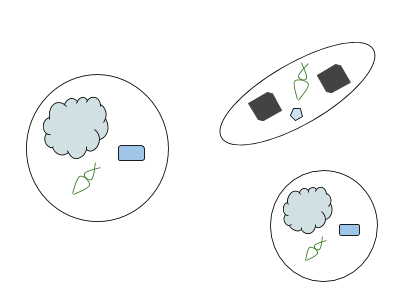
\includegraphics{./img/cellular_structure.png}
\caption{}
\end{figure}

We can create ``things'' with:

\begin{itemize}
\tightlist
\item
  attributes: things those ``things'' have;
\item
  methods: things those ``things'' can do.
\end{itemize}

\begin{figure}[htbp]
\centering
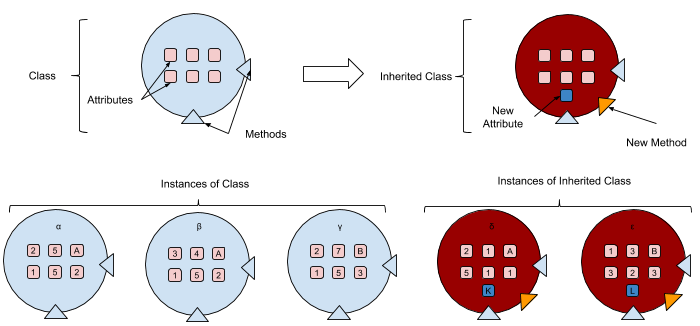
\includegraphics{./img/oop.png}
\caption{}
\end{figure}

\subsection{Defining a class}\label{defining-a-class}

    \begin{Verbatim}[commandchars=\\\{\}]
{\color{incolor}In [{\color{incolor}2}]:} \PY{k}{class} \PY{n+nc}{Student}\PY{p}{(}\PY{p}{)}\PY{p}{:}
            \PY{l+s+sd}{\PYZdq{}\PYZdq{}\PYZdq{}We can create a simple empty class.}
        \PY{l+s+sd}{    }
        \PY{l+s+sd}{    This is a set of rules that says what a student is.}
        \PY{l+s+sd}{    \PYZdq{}\PYZdq{}\PYZdq{}}
\end{Verbatim}

    \begin{Verbatim}[commandchars=\\\{\}]
{\color{incolor}In [{\color{incolor}3}]:} \PY{n}{vince} \PY{o}{=} \PY{n}{Student}\PY{p}{(}\PY{p}{)}  \PY{c+c1}{\PYZsh{} Creating an instance}
        \PY{n}{vince}
\end{Verbatim}

            \begin{Verbatim}[commandchars=\\\{\}]
{\color{outcolor}Out[{\color{outcolor}3}]:} <\_\_main\_\_.Student at 0x7fef0874db70>
\end{Verbatim}
        
    \begin{Verbatim}[commandchars=\\\{\}]
{\color{incolor}In [{\color{incolor}4}]:} \PY{n}{zoe} \PY{o}{=} \PY{n}{Student}\PY{p}{(}\PY{p}{)}  \PY{c+c1}{\PYZsh{} Creating a different instance}
        \PY{n}{zoe}
\end{Verbatim}

            \begin{Verbatim}[commandchars=\\\{\}]
{\color{outcolor}Out[{\color{outcolor}4}]:} <\_\_main\_\_.Student at 0x7fef0874d8d0>
\end{Verbatim}
        
    \subsection{Attributes}\label{attributes}

    \begin{Verbatim}[commandchars=\\\{\}]
{\color{incolor}In [{\color{incolor}8}]:} \PY{k}{class} \PY{n+nc}{Student}\PY{p}{(}\PY{p}{)}\PY{p}{:}
            \PY{n}{courses} \PY{o}{=} \PY{p}{[}\PY{l+s+s2}{\PYZdq{}}\PY{l+s+s2}{Biology}\PY{l+s+s2}{\PYZdq{}}\PY{p}{,} \PY{l+s+s2}{\PYZdq{}}\PY{l+s+s2}{Mathematics}\PY{l+s+s2}{\PYZdq{}}\PY{p}{,} \PY{l+s+s2}{\PYZdq{}}\PY{l+s+s2}{English}\PY{l+s+s2}{\PYZdq{}}\PY{p}{]}
            \PY{n}{age} \PY{o}{=} \PY{l+m+mi}{5}
            \PY{n}{gender} \PY{o}{=} \PY{l+s+s2}{\PYZdq{}}\PY{l+s+s2}{Male}\PY{l+s+s2}{\PYZdq{}}
        \PY{c+c1}{\PYZsh{}Let us now create Vince again:}
        \PY{n}{vince} \PY{o}{=} \PY{n}{Student}\PY{p}{(}\PY{p}{)}
\end{Verbatim}

    Accessing these attributes:

    \begin{Verbatim}[commandchars=\\\{\}]
{\color{incolor}In [{\color{incolor}6}]:} \PY{n}{vince}\PY{o}{.}\PY{n}{courses}
\end{Verbatim}

            \begin{Verbatim}[commandchars=\\\{\}]
{\color{outcolor}Out[{\color{outcolor}6}]:} ['Biology', 'Mathematics', 'English']
\end{Verbatim}
        
    \begin{Verbatim}[commandchars=\\\{\}]
{\color{incolor}In [{\color{incolor}7}]:} \PY{n}{vince}\PY{o}{.}\PY{n}{age}
\end{Verbatim}

            \begin{Verbatim}[commandchars=\\\{\}]
{\color{outcolor}Out[{\color{outcolor}7}]:} 5
\end{Verbatim}
        
    \begin{Verbatim}[commandchars=\\\{\}]
{\color{incolor}In [{\color{incolor}9}]:} \PY{n}{vince}\PY{o}{.}\PY{n}{gender}
\end{Verbatim}

            \begin{Verbatim}[commandchars=\\\{\}]
{\color{outcolor}Out[{\color{outcolor}9}]:} 'Male'
\end{Verbatim}
        
    We can manipulate these attributes just like \textbf{any other} python
variable:

    \begin{Verbatim}[commandchars=\\\{\}]
{\color{incolor}In [{\color{incolor}10}]:} \PY{n}{vince}\PY{o}{.}\PY{n}{courses}\PY{o}{.}\PY{n}{append}\PY{p}{(}\PY{l+s+s2}{\PYZdq{}}\PY{l+s+s2}{Photography}\PY{l+s+s2}{\PYZdq{}}\PY{p}{)}
         \PY{n}{vince}\PY{o}{.}\PY{n}{courses}
\end{Verbatim}

            \begin{Verbatim}[commandchars=\\\{\}]
{\color{outcolor}Out[{\color{outcolor}10}]:} ['Biology', 'Mathematics', 'English', 'Photography']
\end{Verbatim}
        
    \begin{Verbatim}[commandchars=\\\{\}]
{\color{incolor}In [{\color{incolor}11}]:} \PY{n}{vince}\PY{o}{.}\PY{n}{age} \PY{o}{=} \PY{l+m+mi}{28}
         \PY{n}{vince}\PY{o}{.}\PY{n}{age}
\end{Verbatim}

            \begin{Verbatim}[commandchars=\\\{\}]
{\color{outcolor}Out[{\color{outcolor}11}]:} 28
\end{Verbatim}
        
    \begin{Verbatim}[commandchars=\\\{\}]
{\color{incolor}In [{\color{incolor}12}]:} \PY{n}{vince}\PY{o}{.}\PY{n}{gender} \PY{o}{=} \PY{l+s+s2}{\PYZdq{}}\PY{l+s+s2}{M}\PY{l+s+s2}{\PYZdq{}}
         \PY{n}{vince}\PY{o}{.}\PY{n}{gender}
\end{Verbatim}

            \begin{Verbatim}[commandchars=\\\{\}]
{\color{outcolor}Out[{\color{outcolor}12}]:} 'M'
\end{Verbatim}
        
    \subsection{Methods}\label{methods}

    \begin{Verbatim}[commandchars=\\\{\}]
{\color{incolor}In [{\color{incolor}15}]:} \PY{k}{class} \PY{n+nc}{Student}\PY{p}{(}\PY{p}{)}\PY{p}{:}
             \PY{n}{courses} \PY{o}{=} \PY{p}{[}\PY{l+s+s2}{\PYZdq{}}\PY{l+s+s2}{Biology}\PY{l+s+s2}{\PYZdq{}}\PY{p}{,} \PY{l+s+s2}{\PYZdq{}}\PY{l+s+s2}{Mathematics}\PY{l+s+s2}{\PYZdq{}}\PY{p}{,} \PY{l+s+s2}{\PYZdq{}}\PY{l+s+s2}{English}\PY{l+s+s2}{\PYZdq{}}\PY{p}{]}
             \PY{n}{age} \PY{o}{=} \PY{l+m+mi}{5}
             \PY{n}{sex} \PY{o}{=} \PY{l+s+s2}{\PYZdq{}}\PY{l+s+s2}{Male}\PY{l+s+s2}{\PYZdq{}}
         
             \PY{k}{def} \PY{n+nf}{have\PYZus{}a\PYZus{}birthday}\PY{p}{(}\PY{n+nb+bp}{self}\PY{p}{)}\PY{p}{:}
                 \PY{l+s+sd}{\PYZdq{}\PYZdq{}\PYZdq{}This method increments the age of our instance.\PYZdq{}\PYZdq{}\PYZdq{}}
                 \PY{n+nb+bp}{self}\PY{o}{.}\PY{n}{age} \PY{o}{+}\PY{o}{=} \PY{l+m+mi}{1}
\end{Verbatim}

    \begin{Verbatim}[commandchars=\\\{\}]
{\color{incolor}In [{\color{incolor}16}]:} \PY{n}{vince} \PY{o}{=} \PY{n}{Student}\PY{p}{(}\PY{p}{)}
         \PY{n}{vince}\PY{o}{.}\PY{n}{age}
\end{Verbatim}

            \begin{Verbatim}[commandchars=\\\{\}]
{\color{outcolor}Out[{\color{outcolor}16}]:} 5
\end{Verbatim}
        
    \begin{Verbatim}[commandchars=\\\{\}]
{\color{incolor}In [{\color{incolor}17}]:} \PY{n}{vince}\PY{o}{.}\PY{n}{have\PYZus{}a\PYZus{}birthday}\PY{p}{(}\PY{p}{)}
         \PY{n}{vince}\PY{o}{.}\PY{n}{age}
\end{Verbatim}

            \begin{Verbatim}[commandchars=\\\{\}]
{\color{outcolor}Out[{\color{outcolor}17}]:} 6
\end{Verbatim}
        
    \subsection{\texorpdfstring{The \texttt{\_\_init\_\_}
method}{The \_\_init\_\_ method}}\label{the-ux5fux5finitux5fux5f-method}

    \begin{Verbatim}[commandchars=\\\{\}]
{\color{incolor}In [{\color{incolor}18}]:} \PY{k}{class} \PY{n+nc}{Student}\PY{p}{(}\PY{p}{)}\PY{p}{:}
             \PY{k}{def} \PY{n+nf}{\PYZus{}\PYZus{}init\PYZus{}\PYZus{}}\PY{p}{(}\PY{n+nb+bp}{self}\PY{p}{,} \PY{n}{courses}\PY{p}{,} \PY{n}{age}\PY{p}{,} \PY{n}{sex}\PY{p}{)}\PY{p}{:}
                 \PY{l+s+sd}{\PYZdq{}\PYZdq{}\PYZdq{}}
         \PY{l+s+sd}{        What the class should do when it }
         \PY{l+s+sd}{        is used to create an instance}
         \PY{l+s+sd}{        \PYZdq{}\PYZdq{}\PYZdq{}}
                 \PY{n+nb+bp}{self}\PY{o}{.}\PY{n}{courses} \PY{o}{=} \PY{n}{courses}
                 \PY{n+nb+bp}{self}\PY{o}{.}\PY{n}{age} \PY{o}{=} \PY{n}{age}
                 \PY{n+nb+bp}{self}\PY{o}{.}\PY{n}{sex} \PY{o}{=} \PY{n}{sex}
         
             \PY{k}{def} \PY{n+nf}{have\PYZus{}a\PYZus{}birthday}\PY{p}{(}\PY{n+nb+bp}{self}\PY{p}{)}\PY{p}{:}
                 \PY{n+nb+bp}{self}\PY{o}{.}\PY{n}{age} \PY{o}{+}\PY{o}{=} \PY{l+m+mi}{1}
\end{Verbatim}

    \begin{Verbatim}[commandchars=\\\{\}]
{\color{incolor}In [{\color{incolor}19}]:} \PY{n}{vince} \PY{o}{=} \PY{n}{Student}\PY{p}{(}\PY{p}{[}\PY{l+s+s2}{\PYZdq{}}\PY{l+s+s2}{Biology}\PY{l+s+s2}{\PYZdq{}}\PY{p}{,}\PY{l+s+s2}{\PYZdq{}}\PY{l+s+s2}{Math}\PY{l+s+s2}{\PYZdq{}}\PY{p}{]}\PY{p}{,}\PY{l+m+mi}{28}\PY{p}{,}\PY{l+s+s2}{\PYZdq{}}\PY{l+s+s2}{Male}\PY{l+s+s2}{\PYZdq{}}\PY{p}{)}
         \PY{n}{vince}\PY{o}{.}\PY{n}{courses}\PY{p}{,} \PY{n}{vince}\PY{o}{.}\PY{n}{age}\PY{p}{,} \PY{n}{vince}\PY{o}{.}\PY{n}{sex}
\end{Verbatim}

            \begin{Verbatim}[commandchars=\\\{\}]
{\color{outcolor}Out[{\color{outcolor}19}]:} (['Biology', 'Math'], 28, 'Male')
\end{Verbatim}
        
    \subsection{Inheritance}\label{inheritance}

We can use a class to create new classes:

    \begin{Verbatim}[commandchars=\\\{\}]
{\color{incolor}In [{\color{incolor}21}]:} \PY{k}{class} \PY{n+nc}{Math\PYZus{}Student}\PY{p}{(}\PY{n}{Student}\PY{p}{)}\PY{p}{:}
             \PY{l+s+sd}{\PYZdq{}\PYZdq{}\PYZdq{}}
         \PY{l+s+sd}{    A Math student: behaves exactly like a Student }
         \PY{l+s+sd}{    but also has a favourite class attribute.}
         \PY{l+s+sd}{    \PYZdq{}\PYZdq{}\PYZdq{}}
             \PY{n}{favourite\PYZus{}class} \PY{o}{=} \PY{l+s+s2}{\PYZdq{}}\PY{l+s+s2}{Mathematics}\PY{l+s+s2}{\PYZdq{}}
\end{Verbatim}

    \begin{Verbatim}[commandchars=\\\{\}]
{\color{incolor}In [{\color{incolor}23}]:} \PY{n}{becky} \PY{o}{=} \PY{n}{Math\PYZus{}Student}\PY{p}{(}\PY{p}{[}\PY{l+s+s2}{\PYZdq{}}\PY{l+s+s2}{Mathematics}\PY{l+s+s2}{\PYZdq{}}\PY{p}{,} \PY{l+s+s2}{\PYZdq{}}\PY{l+s+s2}{Biology}\PY{l+s+s2}{\PYZdq{}}\PY{p}{]}\PY{p}{,} \PY{l+m+mi}{29}\PY{p}{,} \PY{l+s+s2}{\PYZdq{}}\PY{l+s+s2}{Female}\PY{l+s+s2}{\PYZdq{}}\PY{p}{)}
         \PY{n}{becky}\PY{o}{.}\PY{n}{courses}\PY{p}{,} \PY{n}{becky}\PY{o}{.}\PY{n}{age}\PY{p}{,} \PY{n}{becky}\PY{o}{.}\PY{n}{sex}\PY{p}{,} \PY{n}{becky}\PY{o}{.}\PY{n}{favourite\PYZus{}class}
\end{Verbatim}

            \begin{Verbatim}[commandchars=\\\{\}]
{\color{outcolor}Out[{\color{outcolor}23}]:} (['Mathematics', 'Biology'], 29, 'Female', 'Mathematics')
\end{Verbatim}
        
    \begin{Verbatim}[commandchars=\\\{\}]
{\color{incolor}In [{\color{incolor}25}]:} \PY{c+c1}{\PYZsh{}This class has the methods of the parent class:}
         \PY{n}{becky}\PY{o}{.}\PY{n}{have\PYZus{}a\PYZus{}birthday}\PY{p}{(}\PY{p}{)}
         \PY{n}{becky}\PY{o}{.}\PY{n}{age}
\end{Verbatim}

            \begin{Verbatim}[commandchars=\\\{\}]
{\color{outcolor}Out[{\color{outcolor}25}]:} 31
\end{Verbatim}
        
    \subsection{Summary}\label{summary}

\begin{itemize}
\tightlist
\item
  Classes
\item
  Attributes
\item
  Methods
\item
  Inheritance
\end{itemize}

\subsection{Advantages}\label{advantages}

\begin{itemize}
\tightlist
\item
  Simplicity
\item
  Modularity
\item
  Modifiability
\item
  Extensibility
\item
  Re-usability
\end{itemize}

    \section{Libraries}\label{libraries}

There are a number of built in libraries that extend what Python can do.

    \begin{Verbatim}[commandchars=\\\{\}]
{\color{incolor}In [{\color{incolor}26}]:} \PY{k+kn}{import} \PY{n+nn}{random}
         \PY{n}{random}\PY{o}{.}\PY{n}{seed}\PY{p}{(}\PY{l+m+mi}{0}\PY{p}{)}
         \PY{n}{random}\PY{o}{.}\PY{n}{random}\PY{p}{(}\PY{p}{)}
\end{Verbatim}

            \begin{Verbatim}[commandchars=\\\{\}]
{\color{outcolor}Out[{\color{outcolor}26}]:} 0.8444218515250481
\end{Verbatim}
        
    \begin{Verbatim}[commandchars=\\\{\}]
{\color{incolor}In [{\color{incolor}27}]:} \PY{k+kn}{import} \PY{n+nn}{math}
         \PY{n}{math}\PY{o}{.}\PY{n}{cos}\PY{p}{(}\PY{n}{math}\PY{o}{.}\PY{n}{pi}\PY{p}{)}
\end{Verbatim}

            \begin{Verbatim}[commandchars=\\\{\}]
{\color{outcolor}Out[{\color{outcolor}27}]:} -1.0
\end{Verbatim}
        
    There are also a number of external libraries. This is one of the huge
strengths of Python. Some of these come with Anaconda (the distribution
of Python I recommend):

    \begin{Verbatim}[commandchars=\\\{\}]
{\color{incolor}In [{\color{incolor}28}]:} \PY{k+kn}{import} \PY{n+nn}{sympy}  \PY{c+c1}{\PYZsh{} symbolic mathematics}
         \PY{n}{x} \PY{o}{=} \PY{n}{sympy}\PY{o}{.}\PY{n}{symbols}\PY{p}{(}\PY{l+s+s1}{\PYZsq{}}\PY{l+s+s1}{x}\PY{l+s+s1}{\PYZsq{}}\PY{p}{)}
         \PY{n}{sympy}\PY{o}{.}\PY{n}{diff}\PY{p}{(}\PY{n}{x} \PY{o}{*}\PY{o}{*} \PY{l+m+mi}{2}\PY{p}{,} \PY{n}{x}\PY{p}{)}
\end{Verbatim}

            \begin{Verbatim}[commandchars=\\\{\}]
{\color{outcolor}Out[{\color{outcolor}28}]:} 2*x
\end{Verbatim}
        
    \begin{Verbatim}[commandchars=\\\{\}]
{\color{incolor}In [{\color{incolor}29}]:} \PY{k+kn}{import} \PY{n+nn}{numpy}  \PY{c+c1}{\PYZsh{} Fast numeric computations}
         \PY{n}{A} \PY{o}{=} \PY{n}{numpy}\PY{o}{.}\PY{n}{matrix}\PY{p}{(}\PY{p}{[}\PY{p}{[}\PY{l+m+mi}{0}\PY{p}{,} \PY{l+m+mi}{2}\PY{p}{]}\PY{p}{,} \PY{p}{[}\PY{l+m+mi}{1}\PY{p}{,} \PY{l+m+mi}{2}\PY{p}{]}\PY{p}{]}\PY{p}{)}
         \PY{n}{B} \PY{o}{=} \PY{n}{numpy}\PY{o}{.}\PY{n}{matrix}\PY{p}{(}\PY{p}{[}\PY{p}{[}\PY{l+m+mi}{3}\PY{p}{,} \PY{l+m+mi}{1}\PY{p}{]}\PY{p}{,} \PY{p}{[}\PY{l+m+mi}{1}\PY{p}{,} \PY{o}{\PYZhy{}}\PY{l+m+mi}{2}\PY{p}{]}\PY{p}{]}\PY{p}{)}
         \PY{n}{A} \PY{o}{*} \PY{n}{B}
\end{Verbatim}

            \begin{Verbatim}[commandchars=\\\{\}]
{\color{outcolor}Out[{\color{outcolor}29}]:} matrix([[ 2, -4],
                 [ 5, -3]])
\end{Verbatim}
        
    There are also a number of libraries outside of anaconda that are also
very powerful. Some examples include:

\begin{itemize}
\tightlist
\item
  Ciw: modeling of queues;
\item
  Axelrod: game theory.
\item
  tqdm: adding progress bars to your code :)
\item
  The list is very large\ldots{}
\end{itemize}

To install these libraries from the internet you can open a command
prompt (Windows) or a terminal (Mac OSX) and type:

\begin{Shaded}
\begin{Highlighting}[]
\KeywordTok{pip} \NormalTok{install }\KeywordTok{<}\NormalTok{library-name}\KeywordTok{>}
\end{Highlighting}
\end{Shaded}

    \section{Further resources}\label{further-resources}

There are a number of wonderful resources for learning Python. Here are
some that I have made:

\begin{itemize}
\tightlist
\item
  My first year computing for Mathematics course:
  http://vknight.org/cfm/
\item
  A short set of notebooks that used to teach Mathematics how to use
  Python: https://github.com/drvinceknight/Python-Mathematics-Handbook
\end{itemize}


    % Add a bibliography block to the postdoc
    
    
    
    \end{document}
